\begin{figure}[ht!]
    \centering
    % Top figure (full-width)
    \adjustbox{valign=t}{
        \begin{minipage}{\textwidth} % Full width for the first figure
            \centering
            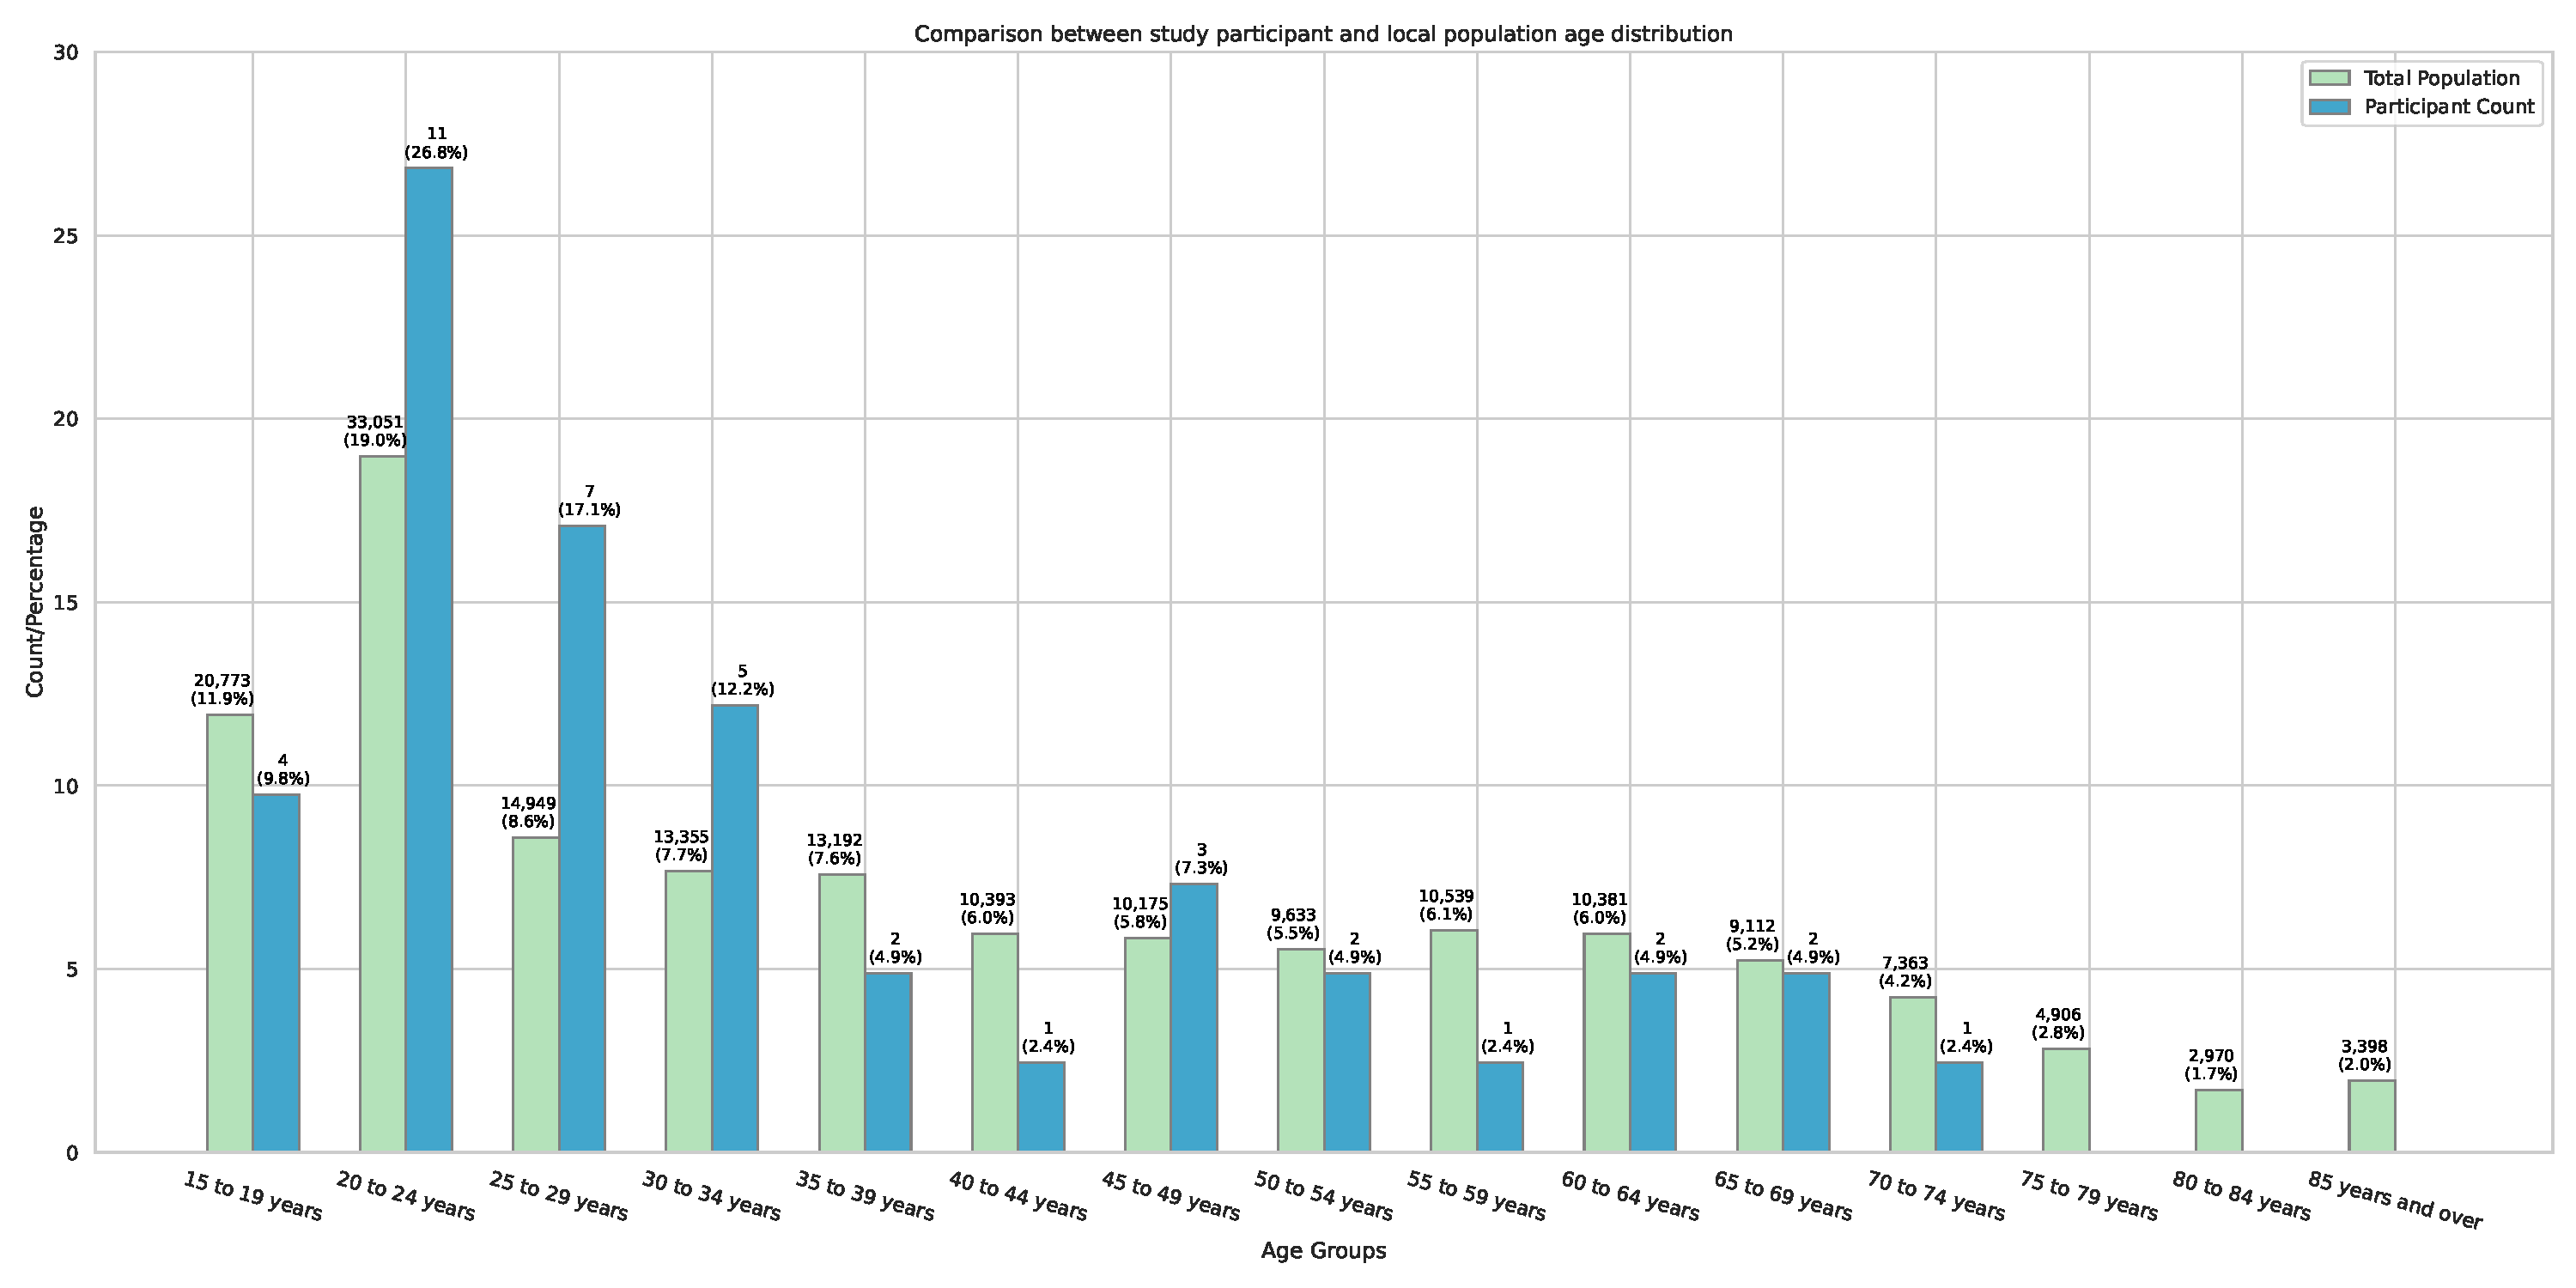
\includegraphics[width=\textwidth, trim=0 13 0 13, clip]{content/image/demo/demo_age_group_vertical.pdf}
            \caption{Age distribution of the study participants were similar to the locale's demographic profile.}
            \label{fig:demoAge}
        \end{minipage}
    }
    
    \vspace{0.25cm} % Add some vertical space between the rows

    % Bottom figures (two figures side by side)
    \adjustbox{valign=t}{
        \begin{minipage}{0.45\textwidth} % First figure on the second row
            \centering
            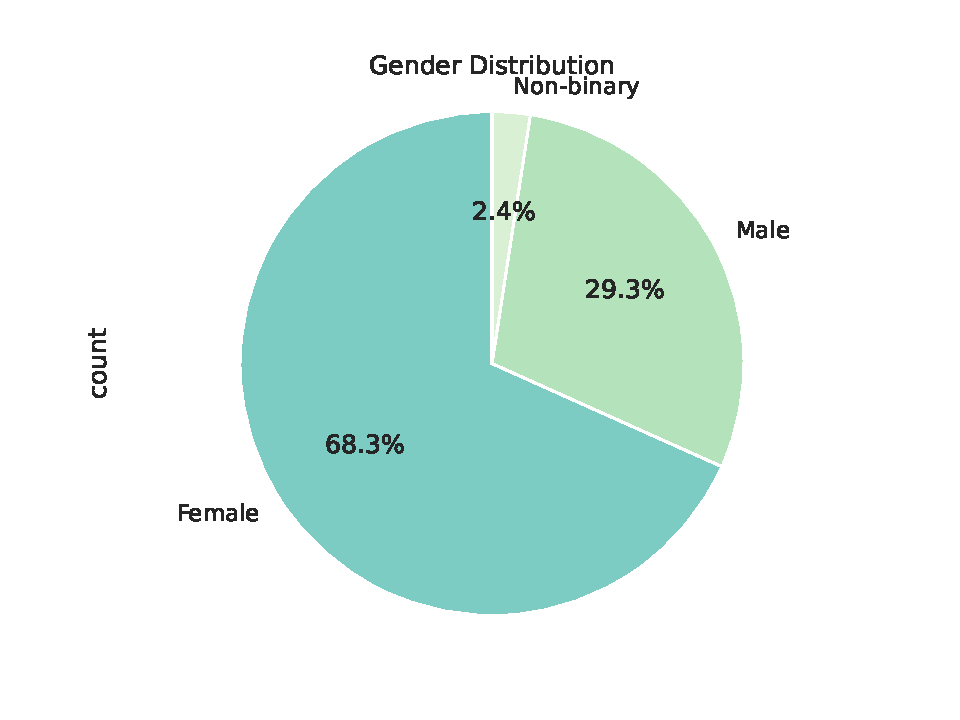
\includegraphics[width=\textwidth]{content/image/demo/demo_gender.pdf}
            \caption{Gender distribution of our participants skewed towards female participants.}
            \label{fig:demoGender}
        \end{minipage}
    }
    \hfill
    \adjustbox{valign=t}{
        \begin{minipage}{0.45\textwidth} % Second figure on the second row
            \centering
            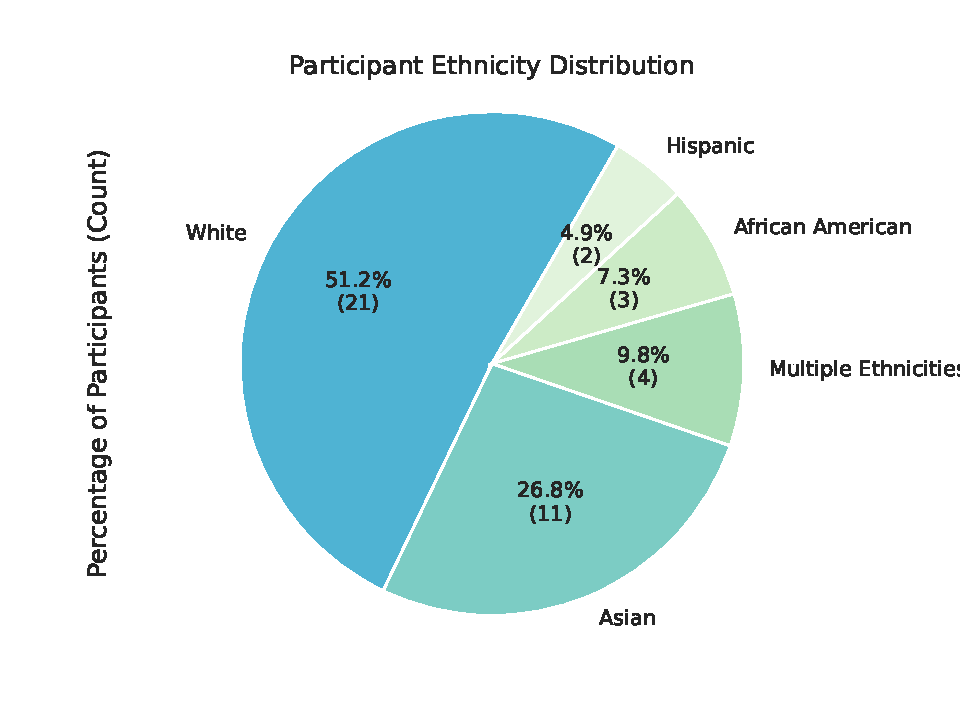
\includegraphics[width=\textwidth]{content/image/demo/demo_ethnicity.pdf}
            \caption{Ethnicity distribution remains diverse with fewer Hispanic and African American participants.}
            \label{fig:demoEthnicity}
        \end{minipage}
    }

    \caption{Demographic distributions: Age, Gender, and Ethnicity}
    \label{fig:Demographics}
\end{figure}

\begin{figure}[ht!]
    \centering
    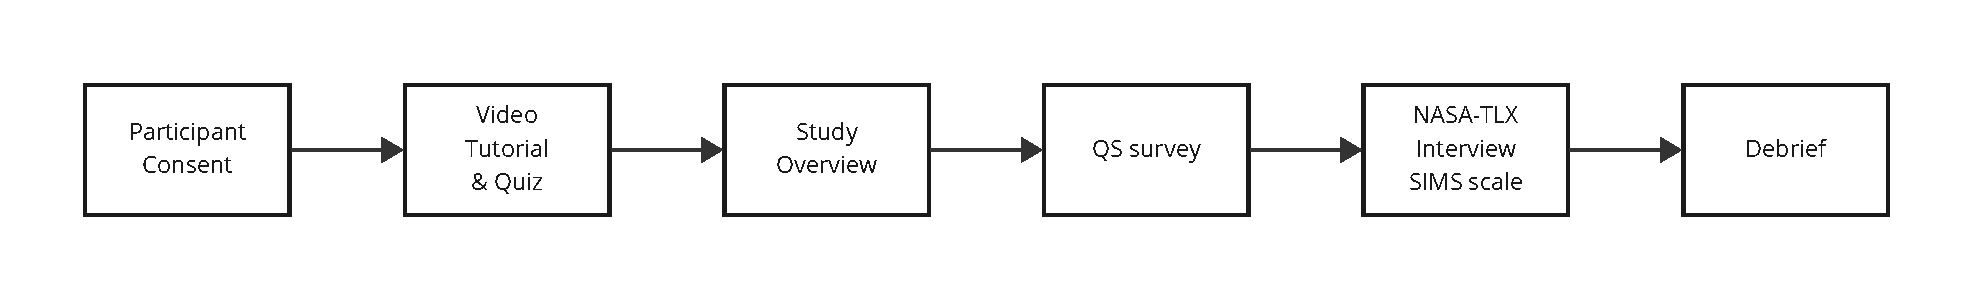
\includegraphics[width=1\textwidth]{content/image/study_flow.pdf}
    \caption{Study protocol: Participants are asked to learn about the mechanism of QS after consenting to the study. The researcher explained the study overview and asked participants to complete the QS. A NASA-TLX survey followed by interviews to understand participants' cognitive load. We debriefed participants after the study.}
    \label{fig:studyProtocol}
\end{figure}

\section{Experiment Design}
\label{sec:experiment}
We recruited $41$ participants, with one excluded\footnote{The participant reported not completing the survey seriously because they believed the experiment was fake.} due to data quality concerns, from a United States college town using online ads, digital bulletins, social media posts, online newsletters, and physical flyers in public spaces beyond campus. To ensure participant diversity, we prioritized non-students by selectively accepting them as we monitored demographics. Study participants' mean age was~$34.63$ years old, with an age distribution similar to the county's demographic profile~(Figure~\ref{fig:demoAge}) albeit a slightly higher representation of younger adults. Gender and race demographics are aggregated in Figure~\ref{fig:demoGender} and~\ref{fig:demoEthnicity}. The study was framed as focusing on societal attitudes to avoid response bias. The university's Institutional Review Board reviewed and approved this study. 
% In the following section we detail the experiment design and rationale.
% If a respondent self-identified as a student, we thanked them and informed them of our current priority for non-students, though some self-identified students were still accepted.
% \subsection{Experiment Protocol}

Figure~\ref{fig:studyProtocol} visually represents the study protocol. Participants completed the study in the lab to control for external influences. Participants used a 32-inch vertical monitor displaying all options. After consenting, participants watched a video explaining the quadratic mechanism without hints of interface operation followed by a quiz to ensure understanding. Participants rewatched the video or consulted the researcher until they could select the correct answers. The participant's screen was captured throughout the study. The researcher primed the participant that the study aimed to help local community organizers understand preferences on societal issues to better allocate resources. Participants were randomly assigned to one of four groups:

\begin{itemize}
    \item Short Text (ST): A text interface with $6$ options. ($N=10$)
    \item Short Two-Phase (SP): A two-phase interface $6$ options. ($N=10$)
    \item Long Text (LT): A text-based interface $24$ options. ($N=10$)
    \item Long Two-Phase (LP): A two-phase interface with $24$ options. ($N=10$)
\end{itemize}

Participants completed the survey independently, without the researcher's presence. They then contacted the researcher for the NASA-TLX survey, followed by a short audio-recorded semi-structured interview. The session concluded with a debriefing and a \$15 cash compensation, during which participants were informed of the study goal on cognitive load and interface design.

We made several experimental design choices. First, we selected a between-subject design to minimize study fatigue, considering the complexity of QS, and avoiding the learning effect that could influence how participants evaluated the options. Second, we chose the context of public resource allotment, where participants expressed their preferences regarding their preference across $6$ or $24$ societal issue options, following the methodology of ~\textcite{chengCanShowWhat2021}. These issues are relevant to all citizens and effectively demonstrate the need to prioritize limited public resources. We curated $26$ societal issues used by Charity Navigator~\cite{CharityNavigator2023} which evaluates over $20,000$ charities in the United States. The interface randomly presents options from this list to participants. Appendix~\ref{sec:charityList} contains the full list.

We decided to test $6$ and $24$ options, representing short and long lists, as identifying the `breaking point' for cognitive overload would require impractical time and resource commitments. Constant sum surveys and the Analytic Hierarchy Process (AHP) recommend fewer than ten and seven options, respectively~\cite{moroneyQuestionnaireDesignHow2019, saatyGroupDecisionMaking2013, saatyPrinciplesAnalyticHierarchy1987}.~\textcite{millerMagicalNumberSeven1956}'s classic work on cognitive processing capacity and~\textcite{saaty2003magic}'s theoretical proof supported the use of $7\pm2$ items. A meta-analysis by~\textcite{chernevChoiceOverloadConceptual2015} identified $6$ and $24$ as common values for short and long lists in choice overload studies, rooted in the original experiment by~\textcite{iyengarWhenChoiceDemotivating2000}.

Finally, we deployed self-report subjective surveys and analytical measures (i.e., time and clickstream data). We adopted the paper-based weighted NASA Task Load Index (NASA TLX), a widely used multidimensional tool that averages six subscale scores to represent overall workload after completing a task~\cite{hart1988development, hartNasaTaskLoadIndex2006, cain2007review}. NASA-TLX is favored for its low cost and ease of administration~\cite{gaoMentalWorkloadMeasurement2013}, with less variability compared to one-dimensional workload scores~\cite{rubioEvaluationSubjectiveMental2004}, making it suitable for our study. Given the extended nature of QS, we did not choose to measured cognitive load using performance measures, psychophysiological measures, subjective measures, and analytical measures~\cite{gaoMentalWorkloadMeasurement2013}

% performance measures using a secondary task were impractical. Psychophysiological measures such as pupil size~\cite{palinkoEstimatingCognitiveLoad2010} and ECG~\cite{haapalainenPsychophysiologicalMeasuresAssessing2010} were costly and sensitive to external factors. 


 % The complexity of QS survey made completing back-to-back studies impractical. Since preferences are constructed, we wanted to ensure that participants were not influenced by their previous preferences, which could affect their perceived cognitive load and decision-making process.

% asking participants to revisit the lab after several days would likely increase dropout rates and demotivate participants from attending in-person sessions. Second, we aimed to reduce the learning effect, which is challenging to eliminate, especially concerning interface operation and decision-making in the survey. 

% Thus, we adopted these values to align with prior research. \footnote{We believe that the original value decision was due to the limitations of the jam flavors.}

% Cognitive load can be measured through performance measures, psychophysiological measures, subjective measures, and analytical measures~\cite{gaoMentalWorkloadMeasurement2013}. Given the extended nature of QS, performance measures using a secondary task were impractical. Psychophysiological measures such as pupil size~\cite{palinkoEstimatingCognitiveLoad2010} and ECG~\cite{haapalainenPsychophysiologicalMeasuresAssessing2010} were costly and sensitive to external factors. 

% Therefore, we deployed self-report subjective surveys and analytical measures (i.e., like time and clickstream data). We adopted the paper-based weighted NASA Task Load Index (NASA TLX), a widely used multidimensional tool that averages six subscale scores to represent overall workload after completing a task~\cite{hart1988development, hartNasaTaskLoadIndex2006, cain2007review}. Despite some criticisms, NASA-TLX is favored for its low cost, ease of administration~\cite{gaoMentalWorkloadMeasurement2013}, and significantly less variability compared to one-dimensional workload scores~\cite{rubioEvaluationSubjectiveMental2004}, making it suitable for our study.


% Finally, participants complete the situational motivation scale (SIMS) to gauge motivation and a demographic survey.
% Last, we describe the two quantitative measurements taken during the study: cognitive load and motivation. 
% , indicating differences in workload definitions among raters within a task and variations in workload sources between tasks

% Tabling SIMS for now. It was not used in the analysis. In addition to NASA-TLX, we administered a situational motivation scale (SIMS) to measure participants' motivation (required citation). We posited that motivation would influence mental demand (required citation). SIMS, chosen for its widespread use, helps understand one's intrinsic motivation, extrinsic motivation, identified regulation, and external regulation, and was originally designed to measure self-determination. Both instruments were administered using pen-and-paper.

% The reason we made this experiment design decision was to minimize . External factors, more prevalent in remote experiments or those conducted via platforms like MTurk, included potential multitasking or interruptions by others. An in-lab study also allowed participants to operate across a consistent device that researchers had full control over.